\par 
Die Umwelt wird in dieser Arbeit als Markov'scher Entscheidungsprozess (\textit{Markov Decision Process, MDP}) angesehen. Dieses Framework findet häufig Verwendung in der stochastischen Kontrolltheorie \cite[S.~3]{Gosavi} und bietet im Bezug auf das \textit{Reinforcement Learning} Problem den mathematischen Rahmen, um u.a. präzise theoretische Aussagen treffen zu können∏ Als \textit{MDP} versteht sich die Formalisierung von sequentiellen Entscheidungsproblemen, bei denen eine Entscheidung nicht nur die sofortige Belohnung beeinflusst, sondern auch alle Folgezustände und somit auch alle zukünftigen Belohnungen \cite[S.~47]{Sutton1998}. Ein Entscheidungsfinder muss somit das Konzept von verspäteten Belohnungen (\textit{delayed rewards}) durchdringen. Vermeintlich schlecht erscheinende Entscheidungen in der Gegenwart können sich im Nachhinein als optimal herausstellen können, angesichts der gesamten Handlung. Ein Skat-Spieler könnte z.B. alle Trümpfe direkt am Anfang spielen, um einen sofortigen Vorteil zu erhalten. Für den Spielausgang ist es aber womöglich besser, die Trümpfe für einen späteren Zeitpunkt aufzubewahren und zu Beginn \glqq schlechte \grqq{} Entscheidungen zu treffen, die dazu führen, ein paar Stiche zu verlieren.
\par 
Probleme, die als \textit{MDP} definiert werden, müssen die Markov-Eigenschaft erfüllen, da diese gewissermaßen als Erweiterung von Markov-Ketten zu betrachten sind, mit dem Zusatz von Aktionen und Belohnungen. Bei den sog. Markov-Ketten führt das System zufällige Zustandswechsel durch \cite[S.~3]{Gosavi}. Dabei sind die Übergangswahrscheinlichkeiten zu den einzelnen Folgezuständen ausschließlich von dem aktuellen Zustand abhängig und nicht aufgrund des historischen Verlaufs \cite[S.~3]{Gosavi}. Da die Markov-Eigenschaft eine essentielle Voraussetzung bei der Problemmodellierung ist, wird sie in Kapitel X näher erläutert. Die Beziehung zwischen Agent und Umwelt, kann durch folgendes Interface dargestellt werden \cite[S.~48]{Sutton1998}:

\par 

\begin{figure}[H]
    \centering
    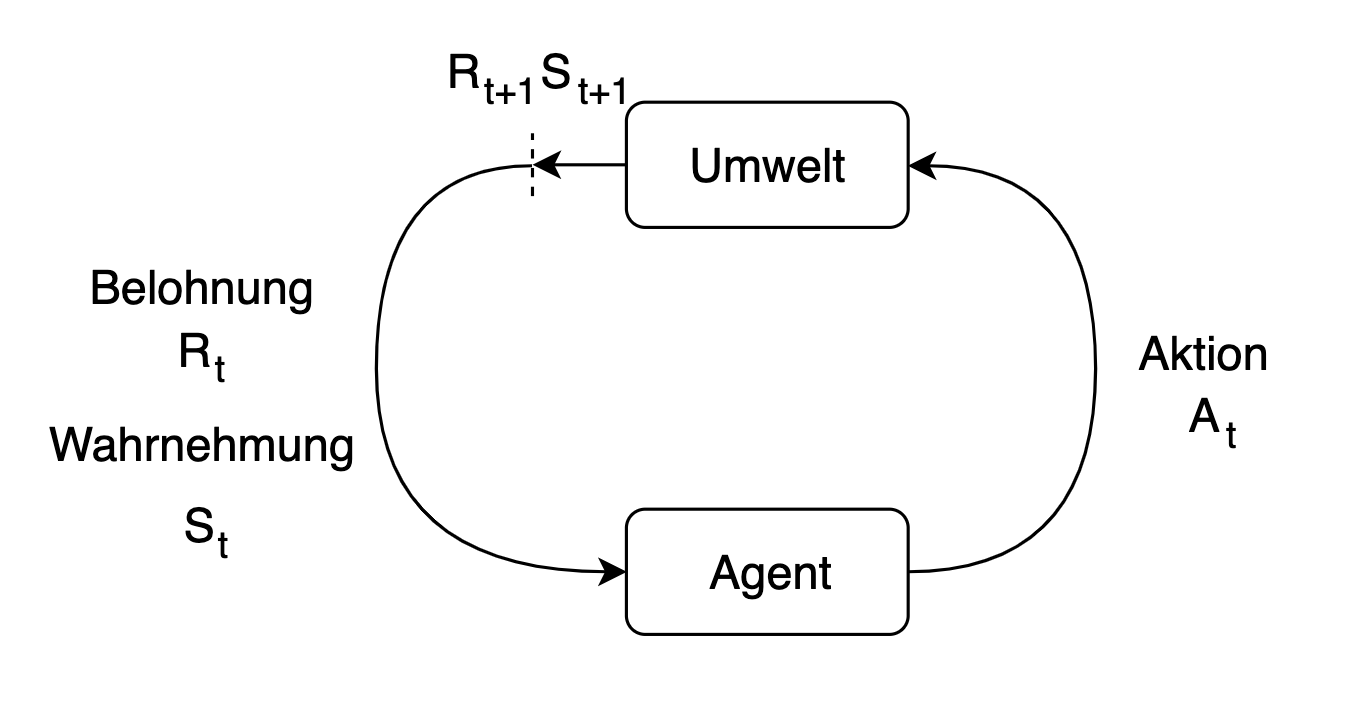
\includegraphics[height=150px]{images/agentUmweltInterface.png}
    \caption{Agent-Umwelt Interface}
\end{figure}


Der Agent interagiert mit dem \textit{MDP} jeweils zu diskreten Zeitpunkten $t = 0, 1, 2, 3, \dots$. \\
Zu jedem Zeitpunkt $t$ beobachtet der Agent den Zustand seiner Umgebung $S_t \in \mathcal{S}$ und wählt aufgrund dessen eine Aktionen $A_t \in \mathcal{A}$. Als Konsequenz seiner Aktion erhält er einen Zeitpunkt später eine Belohnung $R_{t+1} \in \mathcal{R} \subset\mathbb{R} $ und stellt den Folgezustand $S_{t+1}$ fest. 
\par 
In der Literatur findet sich jedoch auch eine abweichende Definition im Bezug auf den Zeitpunkt der Belohnungsvergabe. \cite{watkins1989learning}, \cite{Wiering} und \cite{YuMDP} z.B. binden die Belohnung $R_t$ an das Zustands-Aktions-Paar $(S_t, A_t)$. Die  Definition $R_{t+1}$ bei Aktion $A _{t}$ von \cite{Sutton1998} wird allerdings im Verlauf dieser Arbeit verwendet, da sie besser beschreibt, dass die Belohnung und der Folgezustand gemeinsam berechnet werden und einen Zeitpunkt später, nach Aktion $A_t$, für den Agenten sichtbar sind.
\par 
Das Zusammenspiel zwischen Agenten und MDP erzeugt somit folgende Reihenfolge \cite[~S.48]{Sutton1998}:

\begin{equation}\label{eq:episode}
    S_0, A_0, R_1, S_1, A_1, R_2, S_2, A_2, R_3, \dots
\end{equation}

Wird einfach nur von \textit{MDPs} gesprochen, ist die endliche Variante (\textit{finite MDP}) gemeint, bei dem die Mengen der Zustände, Aktionen und Belohnungen ($\mathcal{S}, \mathcal{A}, \mathcal{R}$) eine endliche Anzahl an Elementen besitzen. In diesem Fall haben die Zufallsvariablen $R_t$ und $S_t$ wohl definierte, diskrete Wahrscheinlichkeitsverteilungen, die nur von dem vorigen Zustand und der vorigen Aktion abhängig sind. Die Wahrscheinlichkeit, dass die bestimmten Werte für diese Variablen $s' \in \mathcal{S}$ und $r \in \mathcal{R}$ eintreten, für einen bestimmten Zeitpunkt $t$ und dem vorigen Zustand $s$ und Aktion $a$, kann somit durch folgende Funktion beschrieben werden \cite[~S.48]{Sutton1998}:

\begin{equation}\label{eq:übergangsfunktion}
p(s',r \mid s,a) \doteq Pr\{S_t=s',R_t=r|S_{t-1}=s,A_{t-1}=a\},
\end{equation}

für alle $s', s \in \mathcal{S}, r \in \mathcal{R}$ und $a \in \mathcal{A}(s)$. Diese Funktion $p$ definiert die sog. Dynamiken (\textit{Dynamics}) eines \textit{MDP}. Sie ist eine gewöhnliche deterministische Funktion mit vier Parametern $p: \mathcal{S} \times \mathcal{R} \times \mathcal{S} \times \mathcal{A} \rightarrow [0,1]$. Das \glqq$\mid$\grqq{} Zeichen kommt ursprünglich aus der Notation für bedingte Wahrscheinlichkeiten, soll hier aber andeuten, dass es sich um eine Wahrscheinlichkeitsverteilung handelt für jeweils alle Kombinationen von $s$ und $a$ \cite[~S.49f]{Sutton1998}:

\begin{equation}\label{eq:wahrscheinlichkeitsverteilung}
\sum_{s' \in \mathcal{S}} \sum_{r \in \mathcal{R}} p(s', r \mid s,a) = 1 \ \forall s \in \mathcal{S}, a \in \mathcal{A}(s)
\end{equation}

Ist das Entscheidungsproblem nicht stochastischer Natur, sondern deterministisch, so ist $p$ immer nur für ein bestimmtes Triplet $(s,a,r)$ für jedes $s' \in \mathcal{S}$ gleich 1, für alle andere jeweils 0. Mit anderen Worten, wird im Zustand $s$ die Aktion $a$ gewählt, führt dies in jedem Fall zu einem bestimmten Folgezustand $s’$. 
\par 

\cite{Sutton1998} erläutern, dass das MDP Framework als extrem flexibel gilt und es demzufolge auf die unterschiedlichsten Probleme angewendet werden kann. Sie führen weiter aus, dass es die nötige Abstraktion für Probleme bietet, bei denen unter Vorgabe eines Ziels mittels Interaktionen gelernt wird. Einzelheiten über das eigentliche Ziel, die Zustände oder die Form des Agenten sind dabei unerheblich. 
Letztendlich kommen die zwei Autoren zu dem Schluss, dass \glqq jedes zielgerichtete Lernen auf drei Signale reduziert werden kann, die zwischen dem Agenten und der Umwelt ausgetauscht werden. Ein Signal repräsentiert die Entscheidung, die der Agent getroffen hat (die Aktion), ein Signal repräsentiert die Basis, auf der er zu dieser Entscheidung gekommen ist (der Zustand) und ein Signal definiert das zu erreichende Ziel (die Belohnung)\grqq{} (S.~50).

